\documentclass[sigconf, nonacm]{acmart}

%%% do not modify the following VLDB block %%%
%%% VLDB block start %%%
\usepackage{pvldb}
%%% VLDB block end %%%

\usepackage{booktabs}
\usepackage{tabularx}
\usepackage{array}
\usepackage{placeins}
\usepackage{tikz}
\usetikzlibrary{arrows.meta,positioning}

\renewcommand\vldbdoi{XX.XX/XXX.XX}
\renewcommand\vldbpages{XXX--XXX}
\renewcommand\vldbavailabilityurl{}

\newcommand{\E}{\mathcal{E}}
\newcommand{\Nom}{\mathsf{Nom}}
\newcommand{\Joint}{\mathsf{Joint}}
\newcommand{\Pess}{\mathsf{PESS}}
\newtheorem{proposition}{Proposition}
\newtheorem{lemma}{Lemma}

\begin{document}
\title{Budgeted Statistics Selection under Uncertain Estimator Policies}

\author{Anonymous Author(s)}
\affiliation{%
  \institution{Anonymous Institution}
  \city{Anonymous City}
  \country{Anonymous Country}
}

\begin{abstract}
Statistics advisors choose which estimation resources to maintain, but the
estimator decides which available resources to use. When its selection policy
is unknown, one resource set can induce different complete estimation schemes
and losses. We formulate budgeted resource selection with a prescribed,
resource-dependent family of admissible schemes and distinguish three
information regimes: a known nominal policy, one unknown policy shared across
tasks, and independent task-wise pessimism. The general maintenance function
is nonnegative and may be nonadditive. For a restricted PostgreSQL 16.14
single-table setting with eligible two-column most-common-value statistics,
we model complete schemes as inclusion-wise maximal matchings and state the
conditions under which this corresponds to the source selector. We prove a
conflict-free certificate under which a nominal optimum is also optimal for
both conservative objectives. Frozen Forest10 evidence gives a six-resource
measured-input instance with distinct nominal and pessimistic optima; its
60-query PostgreSQL follow-up has a small adverse mean difference for the
pessimistic set. On larger Forest10 and Census13 validation instances,
nominal and pessimistic selections coincide at the tested small budgets even
though many raw candidate graphs admit multiple maximal matchings. The
evidence characterizes model sensitivity and selected-set ambiguity; it does
not establish that the prescribed schemes cover every real PostgreSQL choice,
that additive unit budgets measure physical maintenance, or that pessimism
improves query performance.
\end{abstract}

\maketitle

%%% do not modify the following VLDB block %%%
%%% VLDB block start %%%
\vldbtopmatter
%%% VLDB block end %%%

\section{Introduction}

Cardinality estimates shape cost-based query optimization, and their quality
depends on the statistical information maintained by a database. But resource
availability and resource use are separate decisions. An advisor can create
several overlapping statistics while the estimator chooses only a compatible
subset for a particular estimate. That internal choice can depend on
predicate coverage, object eligibility, and tie-breaking. A resource set can
therefore induce more than one complete estimation scheme, with different
estimated cardinalities.

Consider three two-column statistics on attribute pairs $(a,b)$, $(b,c)$,
and $(c,d)$, all built and applicable to a conjunction over four distinct
attributes. A greedy selector that chooses a statistic covering two
unestimated attributes may select $\{ab,cd\}$ or just $\{bc\}$ depending on
candidate order. These are different maximal matchings of the same created
path. A PostgreSQL 16.14 trace fixture observed both outcomes after changing
the statistics-object creation order, under restricted conditions
\cite{pgtrace2026,pgsource1614}. This example motivates a policy-uncertainty
model. It does not imply that a fixed catalog realizes arbitrary matchings or
that the same relation applies to every query form.

We study the advisor's decision when its control ends at resource creation.
The advisor chooses one unordered set of candidate resources shared across
tasks. For each task and each created set, a separately specified family
$\Gamma_i(M)$ describes admissible \emph{complete} schemes. This family is
part of the model: it need not equal the set $\mathcal R_i(M)$ of schemes
realizable by a DBMS. Our main objective sums the worst loss within each
task's prescribed family. The task-wise maxima can require incompatible
internal choices, so this objective need not be the worst outcome of one
shared estimator policy. We also define nominal and shared-policy robust
comparators to make the information assumption explicit.

The generic problem leaves the estimator and maintenance cost abstract. It
does not assume that admissibility is nested as resources are added, or that
maintenance is additive. We instantiate the scheme family for a restricted
PostgreSQL path: eligible two-column MCV objects are labeled edges, and
admissible schemes are maximal matchings of the selected candidate graph. For
a positive pre-clamp multiplicative estimate, the corresponding raw loss is
an absolute signed-log sum. PostgreSQL's rounded and clamped \texttt{Plan
Rows} values remain a separate evaluation measure.

This paper makes three bounded contributions. First, it gives an explicit
model boundary between a global resource decision and task-dependent complete
schemes, including nominal, shared-policy robust, and task-wise pessimistic
objectives. Second, it states a conditional PostgreSQL-to-maximal-matching
correspondence and reports its source premises and fixture-scoped runtime
evidence. Third, it derives a conflict-free sufficient condition for
policy-insensitive optimality and synthesizes frozen studies that exhibit
both policy-sensitive and coincident decisions. We do not present a new
general-purpose solver or claim physical maintenance-cost calibration.

The evaluation asks three narrower questions. Can uncertainty about the
estimator's scheme choice change an optimal resource set on measured inputs?
When it does, do the selected sets behave differently on an already frozen
PostgreSQL cohort? And can structural ambiguity in a workload's candidate
graphs coexist with coincident nominal and pessimistic optima? The evidence
answers each question only for the stated model version, resource budget,
database build, and query cohort. We treat the six-task case as an existence
example and the two larger valid-only fits as counterexamples to the idea
that many ambiguous candidate graphs must imply different selected sets.

The rest of the paper proceeds from the generic decision interface to its
restricted PostgreSQL instance, then gives model-internal results separately
from runtime observations. We end by identifying which assumptions currently
prevent a stronger guarantee or a general claim about optimizer quality.

\begin{figure*}[t]
\centering
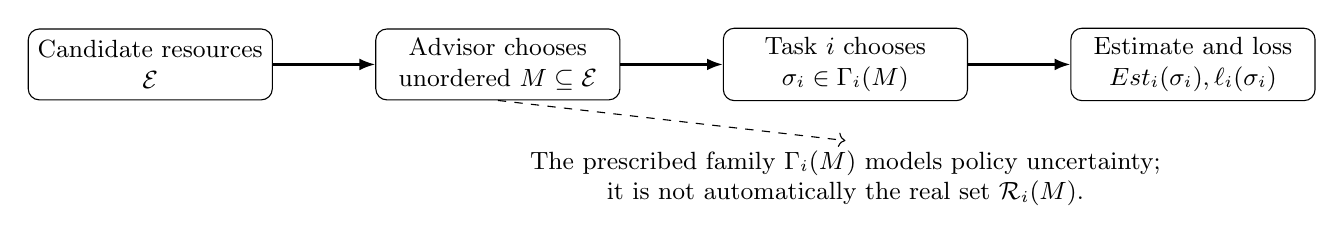
\begin{tikzpicture}[
  box/.style={draw,rounded corners,align=center,minimum height=9mm,
              minimum width=31mm,font=\small},
  arr/.style={-{Latex[length=2mm]},thick}
]
\node[box] (universe) {Candidate resources\\$\E$};
\node[box,right=13mm of universe] (advisor) {Advisor chooses\\unordered $M\subseteq\E$};
\node[box,right=13mm of advisor] (scheme) {Task $i$ chooses\\$\sigma_i\in\Gamma_i(M)$};
\node[box,right=13mm of scheme] (loss) {Estimate and loss\\$\operatorname{Est}_i(\sigma_i),\ell_i(\sigma_i)$};
\draw[arr] (universe) -- (advisor);
\draw[arr] (advisor) -- (scheme);
\draw[arr] (scheme) -- (loss);
\node[font=\small,below=5mm of scheme,align=center] (policy)
  {The prescribed family $\Gamma_i(M)$ models policy uncertainty;\\
   it is not automatically the real set $\mathcal R_i(M)$.};
\draw[dashed,->] (advisor.south) -- (policy.north);
\end{tikzpicture}
\caption{The advisor controls one global created set. The estimator's
task-level scheme choice is modeled separately, and the prescribed
admissibility family is not asserted to equal the real DBMS behavior.}
\Description{A left-to-right flow from the candidate resource universe to the
advisor's unordered created set, then to a task's admissible scheme and its
estimate and loss. A note says the prescribed family need not equal the real
DBMS scheme set.}
\label{fig:decision-boundary}
\end{figure*}

\section{Related Work}

Automatic statistics management selects statistics to improve optimizer
decisions while controlling creation and maintenance overhead
\cite{chaudhuri_narasayya_2000,bruno_chaudhuri_2002}. Work on statistics over
query expressions and conditional selectivity studies how an estimator can
use such information during cardinality estimation
\cite{bruno_chaudhuri_2004}. MAXENT likewise develops a consistent way to
combine partial multivariate information \cite{markl_et_al_2006}. These
papers address resource choice or estimator-side combination; our focus is
the interface between an advisor's created set and the estimator's
resource-dependent complete scheme.

The distinction matters because a statistics-advisor objective usually
evaluates a resource configuration through a workload utility model, while
the estimator's internal use of created objects is often treated as fixed by
the implementation. Here that use is an explicit part of the modeled
outcome. A complete scheme may include the chosen objects and the clauses or
estimator context to which they apply; two schemes can therefore differ even
when both use subsets of the same created set. We do not replace the
estimator-combination mechanisms in prior work. We expose the policy boundary
that a resource-selection analysis would need to specify if such mechanisms
are uncertain to the advisor.

Robustness has also been studied at the query-optimization and physical
design levels. Babcock and Chaudhuri vary cardinality estimates to trade
performance for predictability \cite{babcock_chaudhuri_2005}; El Gebaly and
Aboulnaga incorporate risk and workload generality into physical design
\cite{elgebaly_aboulnaga_2008}. Decision-dependent uncertainty is an
established optimization topic \cite{nohadani_sharma_2018}. These works
motivate explicit uncertainty modeling, but use different decisions,
uncertain quantities, and consequences. We specialize the question to a
resource set whose admissible estimation schemes change with the decision,
and distinguish a shared policy from independent task-wise pessimism.
The distinction between the latter two is consequential: a single unknown
catalog-wide rule couples tasks, whereas task-wise PESS permits each task's
worst admissible scheme to be chosen independently. PESS is thus a conservative
envelope relative to its prescribed families, not a claim that one DBMS
policy realizes all of the maximizing choices simultaneously.

Recent work on robust query optimization studies how an optimizer should
select a plan when cardinality estimates are uncertain; Raychaudhury et al.
construct workload-aware coresets of robust plan candidates
\cite{raychaudhury_et_al_2026}. This line addresses uncertainty at the
plan-choice layer, whereas we study which estimation resources to create
before the estimator chooses a scheme. A practical neighboring system is
EDB's Statistics Advisor: its documentation describes monitoring multi-column
filters, detecting selectivity errors, enumerating extended-statistics
candidates, and weighting them by query benefit and execution cost
\cite{edb_statistics_advisor}. This confirms that workload-aware candidate
selection is an existing advisor function. Our model makes the estimator's
resource-dependent scheme choice explicit as part of the decision analysis;
it does not claim to invent automatic statistics selection.

Cardinality-estimation benchmarks such as AreCEL compare estimator accuracy,
cost, and behavior under changing data \cite{wang_et_al_2021}. Our frozen
evaluation instead examines decisions induced by different policy models.
We keep modeled pre-clamp loss, observed PostgreSQL pre-clamp values, and
rounded/clamped \texttt{Plan Rows} metrics separate. Table~\ref{tab:related}
summarizes these distinctions; the citations identify representative,
not exhaustive, prior work. We make no claim that this paper exhausts the
literature on statistics selection, cardinality estimation, or robust
physical design. The existing decision-dependent uncertainty and graph
optimization literatures provide the general mathematical context; the
present evidence is a scoped integration of that context with one PostgreSQL
estimator path rather than a new general robust-optimization method.

\begin{table*}[t]
\centering
\small
\caption{Representative related work organized by the decision and
uncertainty it studies.}
\label{tab:related}
\begin{tabularx}{\textwidth}{p{2.5cm}p{3.3cm}p{3.2cm}X}
\toprule
Work & Controlled decision & Main uncertainty or choice & Relation to this paper\\
\midrule
Statistics management \cite{chaudhuri_narasayya_2000,bruno_chaudhuri_2002}
& Which statistics to create
& Workload utility and optimizer estimates
& Establishes resource selection; does not use our explicit family of complete schemes.\\
Estimator combination \cite{bruno_chaudhuri_2004,markl_et_al_2006}
& How the estimator combines available information
& Partial or overlapping statistical knowledge
& Studies estimator design; we model its scheme choice from outside.\\
Robust query optimization \cite{babcock_chaudhuri_2005}
& Cardinality estimates and query plans
& Uncertain estimates and plan quality
& Robustness is shared motivation, with a different decision variable.\\
Robust plan coresets \cite{raychaudhury_et_al_2026}
& Candidate query plans
& Uncertain cardinalities and robust plan cost
& Compresses robust plan choices; does not select estimation resources.\\
Robust physical design \cite{elgebaly_aboulnaga_2008}
& Index and physical design selection
& Estimation error and workload shift
& Studies design risk and generality, rather than admissible estimator schemes.\\
Decision-dependent uncertainty \cite{nohadani_sharma_2018}
& Binary decisions in robust optimization
& Uncertainty set depends on decisions
& General optimization context; our $\Gamma_i(M)$ is a finite family of schemes.\\
Practical statistics advising \cite{edb_statistics_advisor}
& Workload-selected extended-statistics candidates
& Multi-column selectivity errors and estimated benefit
& Establishes deployed resource selection; the documentation does not define our scheme-family model.\\
This paper
& One unordered global resource set
& Task-wise complete schemes or one shared policy
& Separates Nominal, Joint, and PESS information regimes.\\
\bottomrule
\end{tabularx}
\end{table*}

\section{Model}

\subsection{Resources, Tasks, and Admissible Schemes}

Let $\mathcal I$ be a finite set of estimation tasks. Task $i$ has true
cardinality $N_i\geq 0$, reference target
$T_i=\max\{1,N_i\}$, and weight $w_i>0$. A task identifies the cardinality
target and its estimation context; it need not be an entire SQL query or a
physical plan node. Let $\E$ be a finite set of candidate estimation
resources. The advisor chooses one global, unordered resource set
$M\subseteq\E$, subject to a maintenance budget.

The generic maintenance function
\[
  \operatorname{Maint}:2^\E\longrightarrow\mathbb R_{\geq0},
  \qquad \operatorname{Maint}(\varnothing)=0
\]
is the additional maintenance cost relative to the baseline database
maintenance process. It may depend on fixed conditions $\xi$, such as
database state, data-modification workload, refresh policy, evaluation
horizon, and accounting convention. We write
$\operatorname{Maint}(M;\xi)$ when exposing those conditions and abbreviate
it as $\operatorname{Maint}(M)$ for a fixed instance. We require
$\operatorname{Maint}(M)\leq B$ for $B\geq0$. No additivity, monotonicity, or
submodularity is assumed.

For each task, let $\Omega_i$ be a finite universe of complete estimation
schemes. A scheme contains enough information to determine the estimate and
has a resource-use set $\operatorname{used}(\sigma)\subseteq\E$. The
scheme may encode selected resources, order, predicate coverage, and
estimator-specific context; it need not itself be a set or a plan. The
prescribed admissibility map is
\[
  \Gamma_i:2^\E\to 2^{\Omega_i}\setminus\{\varnothing\},
  \qquad
  \sigma\in\Gamma_i(M)\Longrightarrow\operatorname{used}(\sigma)\subseteq M.
\]
We require $\Gamma_i(M)\ne\varnothing$ for every task and created set.
There is a baseline scheme in $\Gamma_i(\varnothing)$, but it need not remain
admissible after resources are added. In particular, $\Gamma_i$ need not be
nested. The estimator is a positive-valued map
$\operatorname{Est}_i:\Omega_i\to\mathbb R_{>0}$ and the task loss is any
nonnegative map $\ell_i:\Omega_i\to\mathbb R_{\geq0}$. Our leading
illustration is absolute log error,
\[
  \ell_i(\sigma)=
  \left|\log\frac{\operatorname{Est}_i(\sigma)}{T_i}\right|.
\]
This expression is defined because $T_i\geq1$ and the modeled estimate is
positive. It is a pre-clamp convention; it does not identify PostgreSQL
\texttt{Plan Rows} with the raw estimator value.

The generic estimator map has no assumed additive or multiplicative
structure across resources. Nor does the scheme universe have to consist of
resource subsets: a complete scheme may carry order, fallback, or estimator
state that affects the output even when its selected resource set is the
same. The resource-use consistency condition only says that a scheme cannot
use an uncreated candidate; it does not say that every created candidate is
used or that two schemes with the same used set have the same estimate.

For comparison, let $\mathcal R_i(M)$ denote the set of complete schemes the
deployed system can actually produce under the evaluation conditions. This
real set is an empirical or source-dependent object, not part of the generic
input unless an application supplies it. The formulation requires no
containment between $\mathcal R_i(M)$ and $\Gamma_i(M)$. If every real
outcome is represented by a scheme in $\Gamma_i(M)$ and the same loss is
used, the model's task-wise maximum upper-bounds the real worst-case loss.
Without that inclusion and aligned measurements, PESS is a model objective;
it is not a database guarantee. Equality would be a stronger claim still.

If each SQL query contributes exactly one task, the task set is
query-indexed. A query may instead contribute several logical
cardinality-estimation tasks. A task specifies the target cardinality, a
scheme specifies how available resources and estimator choices produce
that target, and a physical plan specifies execution; these objects are
distinct.

The pessimistic selection problem is
\[
\boxed{
\begin{aligned}
  \min_{M\subseteq\E:\operatorname{Maint}(M)\leq B}\quad
    &F_{\Pess}(M),\\
  F_{\Pess}(M)&=
    \sum_{i\in\mathcal I}w_i
    \max_{\sigma\in\Gamma_i(M)}\ell_i(\sigma).
\end{aligned}
}
\tag{1}
\]
The sum of task-wise maxima need not be attained by one shared policy.
Also, if $\mathcal R_i(M)$ denotes the real set of schemes the DBMS can
produce, no relation between $\mathcal R_i(M)$ and $\Gamma_i(M)$ is implicit.
PESS bounds a real worst-case loss only under an appropriate containment
$\mathcal R_i(M)\subseteq\Gamma_i(M)$ and aligned estimator/loss assumptions.

\subsection{Three Information Regimes}

Suppose a policy parameter $\theta$ induces a complete scheme
$\sigma_i(M;\theta)\in\Gamma_i(M)$ for each task and created set. Let
$\Theta$ be a finite nonempty family of globally shared policies, and let
$\theta_0\in\Theta$ be a known nominal policy. For the same losses and budget
define
\[
\begin{aligned}
F_{\Nom}(M)&=\sum_i w_i\ell_i(\sigma_i(M;\theta_0)),\\
F_{\Joint}(M)&=\max_{\theta\in\Theta}
  \sum_i w_i\ell_i(\sigma_i(M;\theta)),\\
F_{\Pess}(M)&=\sum_i w_i\max_{\sigma\in\Gamma_i(M)}\ell_i(\sigma).
\end{aligned}
\tag{2}
\]
Nominal uses a known policy; Joint assumes one unknown policy is shared by
all tasks; PESS assumes only the task-specific families are justified.
Whenever every policy outcome lies in $\Gamma_i(M)$ and
$\theta_0\in\Theta$, the fixed-set hierarchy
$F_{\Nom}(M)\leq F_{\Joint}(M)\leq F_{\Pess}(M)$ follows. It compares the
same set and modeled estimator, not the separately optimized sets under
actual PostgreSQL outcomes.

The three quantities encode different information available at decision
time. Nominal assumes the advisor knows the reference policy $\theta_0$.
Joint assumes it knows the finite policy family $\Theta$ but not which single
member will govern all tasks. PESS does not require a common policy parameter;
it uses only the per-task envelopes $\Gamma_i(M)$. The hierarchy is
pointwise, before minimizing over $M$. Consequently, the values of the
separately selected solutions need not be ordered when each is evaluated
under a different objective, and the PESS optimizer need not minimize
Nominal loss. The two-task example in Section~\ref{sec:decision-analysis}
will show why the shared and task-wise maxima can differ strictly.

\subsection{Pairwise Maximal-Matching Instance}

For the PostgreSQL instance, each candidate $e\in\E_i$ is a built
two-column MCV object over two distinct attributes. It is represented as a
labeled edge in a graph $H_i=(V_i,\E_i)$; different objects with the same
endpoints remain distinct parallel edges. For a created set $M$,
$H_i[M]$ contains edges in $M\cap\E_i$. A matching is a set of edges with no
shared endpoint. We prescribe
\[
\begin{aligned}
  \Omega_i^{\mathrm{MM}}&=\operatorname{Matchings}(H_i),\\
  \Gamma_i^{\mathrm{MM}}(M)&=
    \operatorname{MaximalMatchings}(H_i[M]).
\end{aligned}
\tag{3}
\]
Maximal means that no available edge can be added; it does not mean
maximum-cardinality. Every finite graph has a maximal matching, and an
edgeless graph has the unique empty matching, so (3) is nonempty for all
$M$. This is a structured instance of (1), not the generic interface.

\section{PostgreSQL Instantiation}

\subsection{When the Selector Is a Greedy Matching Procedure}

The PostgreSQL correspondence is conditional on PostgreSQL 16.14 and a
restricted single-relation AND path. Each relevant clause must be a
supported, simple predicate on one distinct attribute, with exactly one
relevant clause per attribute. Every candidate must be a built two-column
MCV object on that relation, and both of its attribute clauses must remain
eligible for the MCV path. We exclude joins, OR expressions, expression
keys, repeated attributes, multiple relevant clauses on one attribute,
permission exclusions, and other estimators that pre-consume a clause. Under
these assumptions, all currently eligible two-key objects tie on newly
covered attributes and width. The pinned source resolves that tie by
candidate-list order; the list is normally ordered by statistics-object OID.
It then marks the selected clauses consumed and repeats until no candidate
remains \cite{pgsource1614}.

Under this gate, each selected statistic contributes two distinct attribute
vertices. A later eligible statistic can be selected only while both of its
attributes remain available to the MCV estimation path; any shared endpoint
would have been consumed by the earlier selection. The source loop therefore
acts as a priority-ordered greedy procedure on the candidate graph. Its
tie-breaking order selects one matching for a fixed catalog state. The
abstract matching family in (3) ranges over multiple orders to represent
uncertainty about that choice; it should not be read as a randomized runtime
policy or as empirical evidence about the frequency of any matching.

\begin{proposition}[Restricted selector correspondence]
Under the preceding assumptions, the statistics selected by one fixed
PostgreSQL candidate order form a maximal matching of $H_i[M]$.
\end{proposition}
\begin{proof}
Each selected two-column object consumes two distinct clauses. A later
selected object must therefore be disjoint from every earlier one, so the
selected edges form a matching. If an available edge were disjoint from that
matching at termination, both of its clauses would remain unconsumed and it
would still be eligible, contradicting termination. Thus the matching is
maximal.
\end{proof}

Under an arbitrary abstract total priority order, every maximal matching can
be obtained by placing its edges before the other edges.

\begin{proposition}[Abstract order completeness]
Under the same eligibility assumptions, the set of outcomes over all
abstract total priority orders is exactly
$\operatorname{MaximalMatchings}(H_i[M])$.
\end{proposition}
\begin{proof}
The selector correspondence proves that each outcome is a maximal
matching. Conversely, fix a maximal matching $P$ and order its edges before
all other available edges. Each edge of $P$ remains eligible until selected
because $P$ has disjoint endpoints. After its edges have been selected,
maximality implies that every remaining edge meets a covered endpoint, so
the selector stops with exactly $P$.
\end{proof}

Order completeness is a mathematical statement about a freely varying
abstract priority order. It does not say that arbitrary orders are
realizable by changing OIDs in one fixed catalog, or that PostgreSQL's real
possible-scheme set equals (3).

Figure~\ref{fig:path} shows the narrow runtime fixture. An instrumented
PostgreSQL 16.14 build traced selected OIDs and consumed clause indices,
observing $\{ab,cd\}$ in one creation order and $\{bc\}$ in another
\cite{pgtrace2026}. A separate equality-only gate covered path, star,
disconnected, and parallel-edge cases: 26 observations were within the
source-derived gate with no counterexample, two were outside it because an
MCV payload was absent, and four empty-resource observations were
inconclusive because the trace loop was not entered \cite{pg_gate2026}. These
results support the stated scope; they are not universal PostgreSQL evidence.

\begin{figure*}[t]
\centering
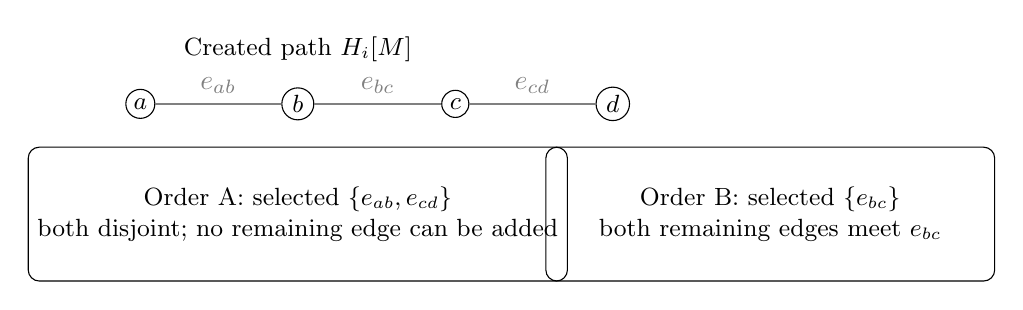
\begin{tikzpicture}[
  v/.style={circle,draw,inner sep=1.5pt,font=\small},
  selected/.style={line width=1.5pt},
  available/.style={line width=.6pt,gray},
  panel/.style={draw,rounded corners,minimum width=57mm,minimum height=17mm,
                align=center,font=\small}
]
\node[v] (a) at (0,1.3) {$a$};
\node[v] (b) at (2,1.3) {$b$};
\node[v] (c) at (4,1.3) {$c$};
\node[v] (d) at (6,1.3) {$d$};
\draw[available] (a)--(b) node[midway,above] {$e_{ab}$};
\draw[available] (b)--(c) node[midway,above] {$e_{bc}$};
\draw[available] (c)--(d) node[midway,above] {$e_{cd}$};
\node[font=\small,above=2mm of b] {Created path $H_i[M]$};
\node[panel] (left) at (2,-.1)
  {Order A: selected $\{e_{ab},e_{cd}\}$\\both disjoint; no remaining edge can be added};
\node[panel] (right) at (8,-.1)
  {Order B: selected $\{e_{bc}\}$\\both remaining edges meet $e_{bc}$};
\end{tikzpicture}
\caption{A single created path has two possible maximal matchings. The
PostgreSQL 16.14 trace fixture observed the two selected sets after changing
statistics-object creation order under the restricted assumptions in the
text. The two panels list outcomes read from traced selected OIDs, not
inferred from \texttt{EXPLAIN}.}
\Description{A four-vertex path with edges ab, bc, and cd, followed by two
observed outcomes: ab and cd under one object order, and bc under another.}
\label{fig:path}
\end{figure*}

\subsection{Positive Pre-Clamp Loss and Maintenance}

For a task with positive baseline pre-clamp estimate $n_i^0$ and positive
single-object correction factors $r_{e,i}$, the model assumes
\[
  \operatorname{Est}^{\mathrm{mult}}_i(P)
    =n_i^0\prod_{e\in P}r_{e,i},\quad
  \alpha_i=\log(n_i^0/T_i),\quad b_{e,i}=\log r_{e,i},
\]
and hence
\[
  \ell_i^{\mathrm{raw}}(P)=
  \left|\alpha_i+\sum_{e\in P}b_{e,i}\right|.
\tag{4}
\]
This is an explicit multiplicative-separability assumption, not an
identity for PostgreSQL. A bounded Forest10 composition check found near
agreement for one disjoint pair but relative residuals $0.1590$ and
$-0.4904$ for two overlapping pairs \cite{issue23_forest10}. The log loss
also requires positive pre-clamp estimates. PostgreSQL's finalized
\texttt{Plan Rows} applies rounding and clamping, so its error is a separate
metric.

For the ordinary finite-positive PostgreSQL regime, the source-scoped
conversion can be represented as
\[
\begin{aligned}
 C_{\mathrm{PG}}(x)&=
 \begin{cases}
  1,&0<x\leq1,\\
  \operatorname{rint}(x),&1<x\leq x_{\max},
 \end{cases}\\
 \ell_i^{\mathrm{plan}}(P)&=
  \left|\log C_{\mathrm{PG}}(\operatorname{Est}^{\mathrm{mult}}_i(P))\right.\\[-2pt]
 &\qquad\left.-\log T_i\right|.
\end{aligned}
\tag{5}
\]
Here $x_{\max}$ is the implementation's finite cap and
$\operatorname{rint}$ follows its floating-point rounding mode. Nonfinite
inputs and separate very-large-value paths are outside this expression.
Raw and plan loss need not have the same optimizer. We use raw
pre-clamp loss for the theoretical model and report finalized Plan Rows only
as a separate observed outcome.

\subsection{Maintenance Cost and Experimental Proxies}

The abstract $\operatorname{Maint}(M)$ in (1) remains nonadditive. For a
controlled PostgreSQL instance, one possible period-level proxy is
\[
  \widehat{\operatorname{Maint}}^{\mathrm{PG}}(M)
     =\sum_{e\in M}\bar m_e,\qquad
  \bar m_e=\nu_{t(e)}p_e(S_{t(e)}),
\tag{6}
\]
where $p_e(S_t)$ denotes candidate-specific CPU work for refreshing object
$e$ from a fixed reference sample of table $t$, and $\nu_t$ is an externally
specified refresh count over the evaluation horizon. This expression is a
model, not an empirical identity. Candidate-specific construction work,
serialization, and attributable catalog work would need separate
measurement; shared sample acquisition and baseline single-column
maintenance are outside the proxy.

Equal positive statistics targets can keep the source-derived requested
sampling requirement unchanged across candidate sets, but they do not force
repeated \texttt{ANALYZE} runs to realize identical random samples. Holding
the tuple values and estimated relation size fixed is a stronger experimental
control; even that does not prove additive CPU time. The coefficients in (6)
have not been calibrated in the reported selection studies. Instead, the
selection experiments use $\bar m_e=1$ and
$B\in\{0,2,3\}$, so the empirical constraint is an object-count proxy.
We report no physical maintenance cost or latency result.

\section{Decision Analysis}
\label{sec:decision-analysis}

\subsection{Pointwise Bounds and a Conflict-Free Certificate}

The hierarchy in (2) follows directly from set inclusion. For a fixed $M$,
the nominal scheme is one member of the shared family, and each shared-policy
scheme is in $\Gamma_i(M)$. Therefore,
\[
F_{\Nom}(M)\leq F_{\Joint}(M)\leq F_{\Pess}(M).
\tag{7}
\]
The inequalities do not order the actual outcomes of the separately selected
sets, and they do not establish a real-system guarantee when the prescribed
families are misspecified.

\begin{lemma}[Conflict-free nominal optimum]
Let $M_{\Nom}$ be a global minimizer of $F_{\Nom}$ over the budget-feasible
sets. If every $\Gamma_i(M_{\Nom})$ is a singleton containing the nominal
scheme, then $M_{\Nom}$ is also a global minimizer of $F_{\Joint}$ and
$F_{\Pess}$, and all three objective values agree at $M_{\Nom}$.
\end{lemma}
\begin{proof}
The singleton condition gives equality of all three objectives at
$M_{\Nom}$. For any feasible $M$, the fixed-set hierarchy and nominal
optimality give
\[
  F_{\Pess}(M)\geq F_{\Joint}(M)\geq F_{\Nom}(M)
  \geq F_{\Nom}(M_{\Nom}).
\]
Thus $M_{\Nom}$ is optimal for both conservative objectives as well.
\end{proof}

In the matching instance it suffices that each $H_i[M_{\Nom}]$ is itself a
matching: its only maximal matching is the set of all its edges (including
the empty case). This is a model-internal sufficient certificate. It does
not say that optimal sets will usually be conflict-free or that every PG
catalog realizes every modeled scheme.

\subsection{Why Shared and Task-Wise Robustness Differ}

Consider two tasks and two overlapping resources $e,f$. With both resources
created, the maximal matchings are $\{e\}$ and $\{f\}$. Let losses for task
1 under $(e,f)$ be $(1,0)$ and for task 2 be $(0,1)$, with unit weights. A
single shared priority selects the same edge for both tasks, so
$F_{\Joint}(\{e,f\})=1$. Independent task-wise maximization selects the
harmful edge separately for each task, giving
$F_{\Pess}(\{e,f\})=2$. Thus PESS is an envelope over task-wise admissible
schemes, not necessarily a realizable global policy.

\begin{figure*}[t]
\centering
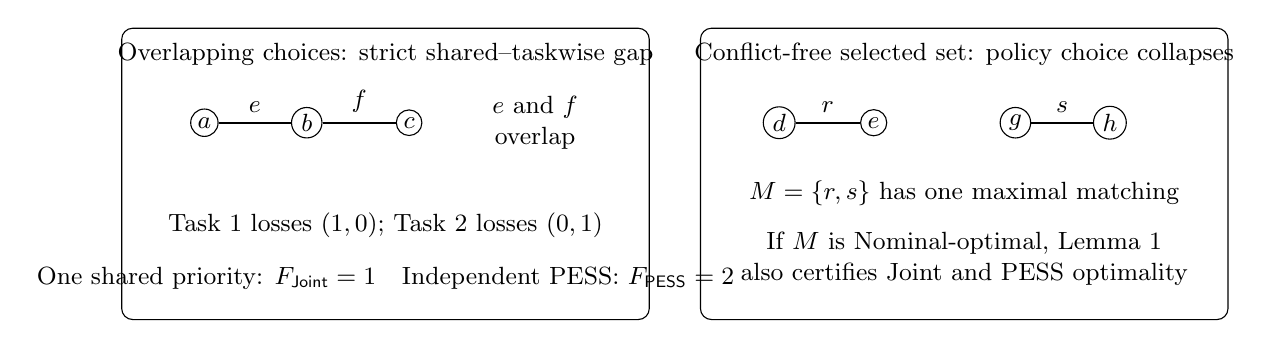
\begin{tikzpicture}[
  v/.style={circle,draw,inner sep=1.3pt,font=\small},
  panel/.style={draw,rounded corners,minimum width=70mm,minimum height=42mm},
  txt/.style={font=\small,align=center}
]
\draw[rounded corners] (-.35,-1.25) rectangle (6.35,2.45);
\node[txt] at (3,2.12) {Overlapping choices: strict shared--taskwise gap};
\node[v] (a) at (.7,1.25) {$a$};
\node[v] (b) at (2.0,1.25) {$b$};
\node[v] (c) at (3.3,1.25) {$c$};
\draw[thick] (a)--node[above,font=\small] {$e$}(b);
\draw[thick] (b)--node[above,font=\small] {$f$}(c);
\node[txt] at (4.9,1.25) {$e$ and $f$\\overlap};
\node[txt] at (3,-.05) {Task 1 losses $(1,0)$; Task 2 losses $(0,1)$};
\node[txt] at (3,-.72) {One shared priority: $F_{\Joint}=1$\quad Independent PESS: $F_{\Pess}=2$};

\draw[rounded corners] (7.0,-1.25) rectangle (13.7,2.45);
\node[txt] at (10.35,2.12) {Conflict-free selected set: policy choice collapses};
\node[v] (d) at (8.0,1.25) {$d$};
\node[v] (e) at (9.2,1.25) {$e$};
\node[v] (g) at (11.0,1.25) {$g$};
\node[v] (h) at (12.2,1.25) {$h$};
\draw[thick] (d)--node[above,font=\small] {$r$}(e);
\draw[thick] (g)--node[above,font=\small] {$s$}(h);
\node[txt] at (10.35,.35) {$M=\{r,s\}$ has one maximal matching};
\node[txt] at (10.35,-.48) {If $M$ is Nominal-optimal, Lemma 1\\also certifies Joint and PESS optimality};
\end{tikzpicture}
\caption{Model-only examples of the information-regime gap and its
conflict-free collapse. In the left panel, one globally shared priority
cannot choose the harmful edge independently for both tasks. In the right
panel, the selected edges have a unique maximal matching; the lemma requires
that this conflict-free set also be a global Nominal optimum. These examples
are mathematical illustrations, not PostgreSQL measurements.}
\Description{Two panels. The first shows overlapping edges e and f and two
tasks whose loss vectors make the shared-policy objective one and the
task-wise pessimistic objective two. The second shows two disjoint selected
edges with a unique maximal matching and notes the conflict-free optimality
certificate.}
\label{fig:policy-examples}
\end{figure*}

The dependence of $\Gamma_i$ on $M$ is also necessary for a nontrivial
worst-case selection objective.

\begin{proposition}[Nested-family degeneracy]
Suppose, for every task $i$, that
$\Gamma_i(M)\subseteq\Gamma_i(M')$ whenever $M\subseteq M'$. Then
$F_{\Pess}(M)\leq F_{\Pess}(M')$. Consequently, the empty set is optimal
for every budget $B\geq0$.
\end{proposition}
\begin{proof}
For each task, the maximum of a nonnegative loss over the smaller family
cannot exceed its maximum over the larger family. Multiplying by $w_i>0$
and summing gives monotonicity. Since
$\operatorname{Maint}(\varnothing)=0\leq B$, the empty set is feasible and
has value no greater than any feasible set.
\end{proof}

Maximal-matching families need not be nested: adding an edge can make an old
complete matching non-maximal. For example, with one available edge $e_{ab}$,
the unique admissible matching is $\{e_{ab}\}$. Add a disjoint edge
$e_{cd}$; the old singleton is no longer maximal, because $e_{cd}$ can be
added, and the new admissible family contains only $\{e_{ab},e_{cd}\}$.
Whether this change raises or lowers the worst loss depends on the task's
losses. Thus the matching instance can violate the nesting premise behind the
degeneracy result, but it does not imply that every resource addition helps
or that every instance has a useful nonempty optimum.

\subsection{Loss Geometry and Inherited Hardness}

For a fixed task and created set, let
\[
  \mathcal M_i(M)=\operatorname{MaximalMatchings}(H_i[M])
\]
and define
\[
  U_i(M)=\max_{P\in\mathcal M_i(M)}\sum_{e\in P}b_{e,i},
  \qquad
  L_i(M)=\min_{P\in\mathcal M_i(M)}\sum_{e\in P}b_{e,i}.
\]
The task's worst raw loss has the endpoint form
\[
  \max_{P\in\mathcal M_i(M)}
  \left|\alpha_i+\sum_{e\in P}b_{e,i}\right|
  =
  \max\{\alpha_i+U_i(M),-\alpha_i-L_i(M)\}.
\tag{8}
\]
This follows from $|x|=\max\{x,-x\}$ and finiteness of
$\mathcal M_i(M)$. The two extrema are over maximal matchings, not ordinary
maximum-weight or maximum-cardinality matchings.

Exact evaluation can inherit the known hardness of minimum maximal
matching \cite{yannakakis_gavril_1980}. Let a graph have $m\geq1$ edges,
make all edges available to one task, and set $b_e=1$ and $\alpha=-m$.
Every maximal matching $P$ has $|P|\leq m$, so its loss is $m-|P|$.
Maximizing the loss therefore computes the minimum cardinality of a maximal
matching. This is a fixed-$M$ hardness observation; it is not a new graph
result or a general classification of the estimator-agnostic problem.

Outer selection can also remain difficult when there is no scheme
uncertainty. With vertex-disjoint candidate edges, every selected set has
one maximal matching and raw loss
$|\alpha+\sum_{e\in M}b_e|$. If integer coefficients are represented
directly, setting $\alpha=-T$, $b_{e_j}=a_j$, and zero maintenance costs
reduces SUBSET SUM on positive integers $a_j$ and target $T$ to deciding
whether some selection has zero loss. This is a representation-scoped
weak-hardness construction: it does not establish a polynomial-time
reduction for every encoding through measured multipliers $r_{e,i}$, and it
says nothing about physical PostgreSQL instances.

\subsection{Computational Scope}

The generic interfaces permit arbitrary finite admissibility maps, losses,
and nonadditive maintenance functions, so complexity depends on the input
representation and evaluation oracles. The preceding reductions explain why
an unrestricted tractability claim would be inappropriate. We do not claim
an algorithmic speedup in this paper.

\section{Evaluation}

\subsection{Evidence and Comparison Protocols}

We synthesize already frozen evidence; this paper reports no new PostgreSQL
run, refit, or optimization solve. Each study has a different role and
model version. Issue~\#23 used six Forest10 valid tasks, six adjacent
resources, positive pre-clamp measurements from a fixed sample, 18-decimal
rationalized log coefficients, one-unit costs, and exact exhaustive
references. Its result is exact for that rationalized finite instance, not
for the original floating-point measurements. Issue~\#38 then compared the
resulting budget-three sets on 60 frozen Forest10 test IDs, two repetitions
per ID, in PostgreSQL 16.14; it reports observed pre-clamp estimates and
catalog payloads \cite{issue23_forest10,issue38_heldout}.

The six selection tasks are a deterministic construction sample rather than
a workload-frequency sample. Table~\ref{tab:anchors} records their source
query suffixes and truth cardinalities. The zero-truth task is retained with
$T_i=1$; no task was replaced or removed to make the logarithm convenient.
For each task, the calibration protocol measured the baseline and every
candidate object twice after replaying the same fixed sample. The resulting
84 records provide the per-task model inputs, but do not constitute a sample
of all queries eligible for pairwise MCV statistics.

\begin{table}[t]
\centering
\small
\caption{Six Forest10 valid-query anchors used for the Issue~\#23
construction sample. Each query remains a separate task, including the
zero-truth task with target floor $T_i=1$ \cite{issue23_forest10}.}
\label{tab:anchors}
\begin{tabular}{lrrr}
\toprule
Anchor object & Query ID suffix & $N_i$ & $T_i$\\
\midrule
$e_{01}$ & 000005 & 3 & 3\\
$e_{12}$ & 000003 & 0 & 1\\
$e_{23}$ & 000009 & 119,625 & 119,625\\
$e_{34}$ & 000001 & 343 & 343\\
$e_{45}$ & 000010 & 12,916 & 12,916\\
$e_{56}$ & 000011 & 8 & 8\\
\bottomrule
\end{tabular}
\end{table}

The larger Forest10 model uses all 10,000 valid tasks and a corrected-log
model; its B=0/2/3 exact selections are compared with an official test split
using ordinary \texttt{Plan Rows}. Census13 uses a distinct
\texttt{clamped-log-v2} model and a separate valid-only order-sensitivity
analysis. Its Nominal enumeration across ten frozen orders was compared to
the already frozen PESS result; it is not a PostgreSQL or test-set
comparison \cite{issue64_forest10,issue71_census13}. Separately, the
Issue~\#59 structure audit used 10,000 valid queries per dataset without
reading truth or running PostgreSQL \cite{issue59_structure}.

Across these comparisons, exactness refers to Fraction/reference
calculations for recorded rationalized model inputs. It does not upgrade
floating-point PostgreSQL values or solver status into exact model inputs,
and it does not imply exact physical semantics. Candidate-graph ambiguity,
model-level selected sets, pre-clamp observations, and rounded/clamped
\texttt{Plan Rows} are reported as distinct evidence layers.

\paragraph{Provenance boundaries.}
The papers and results below are a synthesis of frozen, previously executed
work. The Issue~\#23 and Issue~\#38 PostgreSQL records were author-reported
local measurements; the source reports retain exact build commits, frozen
inputs, commands, outputs, and limits. The full-valid Forest10 evaluation
uses a separate PostgreSQL build and same-run sample. The Census13 table is
an exact model comparison only. Table~\ref{tab:provenance} summarizes the
distinctions needed to interpret the results.

\begin{table*}[t]
\centering
\small
\caption{Source, split, model, and output provenance for the frozen studies
used in this paper. Detailed commands, hashes, and raw-record locations are
in the cited reports.}
\label{tab:provenance}
\begin{tabularx}{\textwidth}{p{2.2cm}p{3.6cm}p{4.0cm}X}
\toprule
Study & Input and environment & Model or metric & Evidence boundary\\
\midrule
PG selector trace
& PostgreSQL 16.14; pinned source tag and instrumented development build
& Traced selected OIDs and consumed clause indices on controlled fixtures
& Conditional source claim; fixture-level runtime observations only.\\
Issue 23/38
& AreCEL Forest10; six valid selection tasks and 60 frozen test IDs;
PostgreSQL 16.14 at the recorded research commit
& Rationalized raw pre-clamp log model; held-out raw pre-clamp errors
& Construction sample and bounded cohort; repeated observations are paired by query ID.\\
Issue 59
& Forest10 and Census13 official 10,000-query valid splits; no truth reads or PostgreSQL
& Raw graph ambiguity and strict pairwise syntax eligibility
& Describes candidate-graph structure, not built MCV payloads or realized selection.\\
Issue 64
& Forest10: 10,000 valid and 10,000 official test queries; fresh PostgreSQL 16.14 build for test evaluation
& Corrected-log valid-only decisions; test \texttt{Plan Rows} and Q1
& Nominal/PESS sets coincide; official-split result has template overlap and prior exposure.\\
Issue 71
& Census13 10,000 valid tasks and existing full-valid observations
& Separate \texttt{clamped-log-v2} model; ten Nominal priority orders
& PESS comparison reuses the frozen baseline; no test evaluation or PostgreSQL claim.\\
\bottomrule
\end{tabularx}
\end{table*}

\paragraph{Metric definitions.}
For positive pre-clamp estimates, the primary observed loss is
$|\ln(\widehat N/T)|$ with $T=\max(1,N)$. The Issue~\#38 report pools
120 repetitions per resource set for distributional summaries, and also
averages repetitions within each of 60 query IDs for paired counts. The
Issue~\#64 \texttt{Plan Rows} Q1 ratio is
\[
  Q1(\widehat N,N)=
  \frac{\max\{\widehat N,N,1\}}{\max\{\min(\widehat N,N),1\}},
\tag{9}
\]
and its quantiles use nearest rank over 10,000 queries. The reported mean
absolute log error uses only query pairs with positive estimate and truth.
Q1 is finite when either input is zero, but it is not the primary
pre-clamp loss. Neither metric measures plan quality or latency.

\subsection{Scoped PostgreSQL Selector Evidence}

The runtime reports support a maximal-matching correspondence under a
strict gate, not unrestricted coverage. Table~\ref{tab:pg-gate} summarizes
the equality-only gate's classification and the separate path trace.

\begin{table}[t]
\centering
\small
\caption{Frozen PostgreSQL 16.14 selector evidence. The gate is
source-derived under the recorded eligibility premises; the path outcomes
are directly traced fixture observations.}
\label{tab:pg-gate}
\begin{tabular}{lr}
\toprule
Observation class & Count\\
\midrule
Within-gate maximal-matching pass & 26\\
Within-gate counterexample & 0\\
Outside gate (no built MCV payload) & 2\\
Inconclusive (empty setup bypassed trace loop) & 4\\
\midrule
Path fixture outcome, order A & $\{ab,cd\}$\\
Path fixture outcome, order B & $\{bc\}$\\
\bottomrule
\end{tabular}
\end{table}

The equality-only gate used a deterministic fixture with 20,000 rows and
eight labeled candidates. It covered ten equality queries and eleven
setup/order combinations, each repeated twice. The resulting ledger
reconciled 32 outcomes. Candidate consideration was inferred from pinned
source control flow under the recorded premises; instrumentation did not
independently trace every rejected candidate. The separate path fixture
directly traced selected OIDs and consumed clause indices. Neither study
establishes that every real possible scheme is represented in the prescribed
family for general PostgreSQL workloads.

\paragraph{Observed graph forms.}
The equality-only gate exercised four graph forms in addition to controls.
Table~\ref{tab:topologies} gives selected sequences under its two catalog
orders. The path and disconnected pair selected the same resource sets in
both orders, while the star and parallel-edge cases produced different
maximal matchings. Each listed order was repeated twice; these are bounded
fixture observations, not a frequency estimate over PostgreSQL workloads.

\begin{table*}[t]
\centering
\small
\caption{Selected statistics sequences from four Issue~\#47 Stage~2A
topologies. Positive-MCV selections were reconciled with the source-derived
candidate ledger; the fixture does not establish arbitrary order
realization in a fixed catalog \cite{pg_gate2026}.}
\label{tab:topologies}
\begin{tabularx}{\textwidth}{p{2.4cm}p{3.2cm}p{3.6cm}X}
\toprule
Topology & Available labeled edges & Catalog order 1 & Catalog order 2\\
\midrule
Three-edge path & $\{e_{01},e_{12},e_{23}\}$ &
 $e_{01}\to e_{23}$ & $e_{23}\to e_{01}$\\
Three-edge star & $\{e_{01},e_{12},e_{13}\}$ &
 $e_{01}$ & $e_{13}$\\
Disconnected pair & $\{e_{01},e_{34}\}$ &
 $e_{01}\to e_{34}$ & $e_{34}\to e_{01}$\\
Parallel labeled pair & $\{e_{01},p_{01}\}$ &
 $e_{01}$ & $p_{01}$\\
\bottomrule
\end{tabularx}
\end{table*}

\subsection{A Policy-Sensitive Six-Resource Instance}

Table~\ref{tab:issue23} separates exact model decisions from PostgreSQL
outcomes. Exhaustive reference enumeration of the Issue~\#23 rationalized
model found policy-sensitive selections at budgets three and five. The
displayed objective values are rounded decimals of exact rational reference
values; values from different policy objectives are not held-out prediction
metrics and should not be ranked as if they measured the same quantity.

The six-task model was built from six Forest10 valid queries selected by a
fixed earliest-unused rule. PostgreSQL 16.14 was run twice for the baseline
and each of six candidate objects using one replayed reference sample; the
frozen calibration contains 84 task/candidate/repetition records. Objects
$e_{12},e_{23},e_{34}$ each had 300 MCV items, whereas $e_{01},e_{45},e_{56}$
had no MCV payload in that sample. The raw positive estimates were converted
to natural logs with high-precision Decimal arithmetic, quantized to 18
decimal places, and stored as exact Fractions. The experiment enumerated all
720 common candidate orders for the Joint model and used exhaustive resource
selection with independent objective verification \cite{issue23_forest10}.

The same report checked how single-object factors compose for three
two-object configurations. For the disjoint pair $e_{12}+e_{34}$, PostgreSQL
selected both objects and the product prediction differed from the observed
pre-clamp value by relative $-1.84\times10^{-16}$. For overlapping pairs
$e_{12}+e_{23}$ and $e_{23}+e_{34}$, the selector used only one object and
the product predictions had relative residuals $0.1590$ and $-0.4904$.
These observations limit the multiplicative model; they do not show that
all disjoint pairs compose exactly.

The 84-record calibration led to a sharp separation between requested
resources and effective MCV objects in this fixed sample: $e_{12}$,
$e_{23}$, and $e_{34}$ each had 300 MCV items, while $e_{01}$, $e_{45}$,
and $e_{56}$ had none. The model still retained all six candidate resources
as available choices, because payload realization belongs to the observed
PostgreSQL layer rather than the abstract candidate-set definition. This
gap is material at budget three: the model's pessimistic choice includes
$e_{01}$, but the held-out catalog snapshots did not provide an effective
two-column MCV payload for it.

\begin{table*}[t]
\centering
\small
\caption{Frozen Forest10 PostgreSQL MCV payload and two-object composition
observations from one fixed sample. Residual is the relative difference
between the product prediction and observed pre-clamp estimate
\cite{issue23_forest10}.}
\label{tab:composition}
\begin{tabular}{lll}
\toprule
\multicolumn{3}{c}{(a) Single-object MCV payloads}\\
\midrule
Candidate objects & MCV item count & Observed status\\
\midrule
$e_{01},e_{45},e_{56}$ & 0 / absent & No effective MCV payload\\
$e_{12},e_{23},e_{34}$ & 300 each & Built MCV payload\\
\midrule
\multicolumn{3}{c}{(b) Two-object composition on one valid task}\\
\midrule
Created subset & PG-selected objects & Product residual\\
\midrule
$e_{12}+e_{34}$ & Both & $-1.84\times10^{-16}$\\
$e_{12}+e_{23}$ & One object & $0.1590$\\
$e_{23}+e_{34}$ & One object & $-0.4904$\\
\bottomrule
\end{tabular}
\end{table*}

\begin{table*}[t]
\centering
\small
\caption{Issue~\#23 exact reference decisions and Issue~\#38 held-out
PostgreSQL measurements are separate evidence panels. Values in panel (a)
are rounded displays of exact rational objectives for the rationalized
instance. Panel (b) summarizes 120 repeated measurements per deployment;
paired counts average the two repetitions within each of 60 query IDs.}
\label{tab:issue23}
\begin{tabular}{rp{4.2cm}p{4.2cm}p{5.4cm}}
\toprule
\multicolumn{4}{c}{(a) Exact reference selections for the six-task model}\\
\midrule
B & Nominal set (native objective) & Joint/PESS set (native objective) & Relation\\
\midrule
$0$ & $\varnothing$ (14.672700) & $\varnothing$ (14.672700) & Same set\\
$2$ & $\{e_{01},e_{34}\}$ (13.498446) & $\{e_{01},e_{34}\}$ (13.498446) & Same set\\
$3$ & $\{e_{12},e_{23},e_{34}\}$ (13.303092) & $\{e_{01},e_{34}\}$ (13.498446) & Distinct sets\\
$5$ & $\{e_{12},e_{23},e_{34}\}$ (13.303092) & $\{e_{01},e_{34}\}$ (13.498446) & Distinct sets\\
\midrule
\multicolumn{4}{c}{(b) Frozen PostgreSQL held-out comparison ($n=120$ repeated rows per set)}\\
\midrule
Selected set & MCV payloads & Trace rows & Mean / median / P90 / max log error\\
\midrule
Empty & None & $0/120$ & 5.02104 / 2.55550 / 12.79932 / 33.44741\\
Nominal $\{e_{12},e_{23},e_{34}\}$ & $e_{12},e_{23},e_{34}$ & $114/120$ &
 4.92783 / 2.55728 / 12.79932 / 33.44741\\
PESS $\{e_{01},e_{34}\}$ & $e_{34}$ & $94/120$ &
 4.95206 / 2.47246 / 12.79932 / 33.44741\\
\bottomrule
\end{tabular}
\end{table*}

At budget three, the nominal optimum has model objective $13.303092$ but a
task-wise PESS value of $14.320234$ on that same set. The pessimistic optimum
$\{e_{01},e_{34}\}$ has PESS value $13.498446$, so the nominal set's exact
rational PESS regret rounds to $0.821788$ for display. The nominal set
remains optimal for its own objective at budgets
three and five, while the Joint and PESS choices remain $\{e_{01},e_{34}\}$.
This is the measured-input instance in which the nominal decision differs
from the two conservative regimes; the displayed magnitudes are native
model objectives, not comparable to the PostgreSQL held-out mean below.

The set geometry clarifies why the model decisions separate. At $B=3$, the
Nominal set $\{e_{12},e_{23},e_{34}\}$ forms a three-edge path and admits two
maximal matchings, $\{e_{12},e_{34}\}$ and $\{e_{23}\}$. The selected
Joint/PESS set $\{e_{01},e_{34}\}$ is conflict-free and therefore has a
singleton maximal-matching family in this instance. It removes the model's
within-task choice while trading away Nominal objective value. This is
consistent with the conflict-free certificate, although the certificate
alone does not predict which conflict-free set the optimizer will choose.
The budgets are upper bounds under unit object-count cost: at $B=5$ the
optimizers still choose only three resources, so the additional capacity is
not forced to be used.

The paired query-level comparison has 34 IDs with higher PESS error, 11 with
lower error, and 15 ties; the mean difference is $+0.02422$ for PESS minus
Nominal. The requested
$e_{01}$ object had no effective MCV payload in the fixed-sample snapshots;
thus the physical PESS deployment did not realize every correction assumed
by the model. Figure~\ref{fig:paired} displays the 60 query-level
comparisons. The result is a bounded adverse price-of-pessimism example, not
a population ranking, significance claim, or evidence that PESS generally
harms estimates.

\begin{figure}[t]
\centering
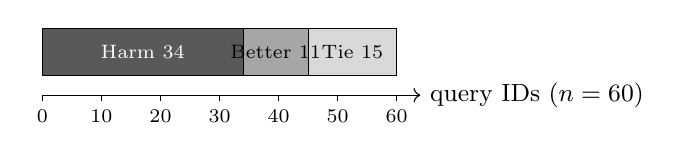
\begin{tikzpicture}[x=0.075cm,y=1cm]
\draw[->] (0,0)--(64,0) node[right,font=\small] {query IDs ($n=60$)};
\draw[fill=black!65] (0,.25) rectangle (34,.85);
\draw[fill=black!35] (34,.25) rectangle (45,.85);
\draw[fill=black!15] (45,.25) rectangle (60,.85);
\node[font=\scriptsize,text=white] at (17,.55) {Harm 34};
\node[font=\scriptsize] at (39.5,.55) {Better 11};
\node[font=\scriptsize] at (52.5,.55) {Tie 15};
\foreach \x in {0,10,20,30,40,50,60}
  {\draw (\x,0)--(\x,-.07) node[below,font=\scriptsize] {\x};}
\end{tikzpicture}
\caption{PESS minus Nominal error after averaging the two repetitions within
each held-out query ID. Counts are descriptive paired outcomes, not
independent repetitions or a significance test \cite{issue38_heldout}.}
\Description{A stacked horizontal bar for 60 query IDs: PESS has higher error
on 34, lower error on 11, and equal error on 15.}
\label{fig:paired}
\end{figure}

\subsection{Ambiguity in Candidate Graphs and Selected Sets}

Table~\ref{tab:larger} contrasts graph-level opportunities with frozen
small-budget optima. The ambiguity percentages are computed on the raw
candidate graphs for the full 10,000-query validation split. Strictly
eligible Stage~2B query counts are much smaller. Neither raw graph ambiguity
nor query syntax establishes built PostgreSQL MCV payloads or realized
scheme choice.

\begin{table*}[t]
\centering
\small
\caption{Raw validation-graph ambiguity and frozen valid-only selections.
Forest10 uses a corrected-log model; Census13 uses the separately versioned
\texttt{clamped-log-v2} model. Their numeric objectives are not pooled.}
\label{tab:larger}
\begin{tabularx}{\textwidth}{p{1.8cm}p{2.5cm}p{2.5cm}p{3.4cm}X}
\toprule
Dataset/model & Raw graphs with $\geq2$ maximal matchings & Strict eligible
queries & Unique frozen selections & Nominal/PESS comparison\\
\midrule
Forest10, corrected-log
& 4,749/10,000 (47.49\%)
& 135/10,000 (1.35\%)
& $B=0:\varnothing$; $B=2:\{e_{01\_06},e_{02\_07}\}$; $B=3$ adds $e_{03\_04}$
& Same unique exact Nominal and PESS sets at $B=0,2,3$.\\
Census13, clamped-log-v2
& 4,627/10,000 (46.27\%)
& 58/10,000 (0.58\%)
& $B=0:\varnothing$; $B=2:\{e_{02\_03},e_{04\_06}\}$; $B=3$ adds $e_{01\_05}$
& Ten Nominal orders had the same unique optima; these equal the frozen PESS sets.\\
\bottomrule
\end{tabularx}
\end{table*}

For the tested budgets, every nonempty winning set in both datasets contains
mutually vertex-disjoint resource edges, so each selected instance has a
unique maximal matching. This explains how the chosen configurations can
remove modeled policy ambiguity even when many full candidate graphs are
ambiguous. For Census13, the PESS result was reused from the frozen
schema-order baseline rather than recomputed in the ten-order run. These
findings are model-internal, not PostgreSQL traces or held-out PESS effects.

For these frozen outputs, the conflict-free condition supplies a direct
model-internal explanation for Nominal/PESS agreement. A set of pairwise
disjoint selected edges has exactly one maximal matching in every task graph
that contains those edges, so all modeled schemes collapse to the same
resource-use set. When the Nominal optimizer returns such a globally
optimal set, the lemma in Section~\ref{sec:decision-analysis} certifies it
as optimal for Joint and PESS as well. This certificate is available after
the selected set is known; it does not show that a generic optimizer will
find a conflict-free optimum or that graph ambiguity elsewhere in the
candidate universe is harmless to every decision.

The Forest10 corrected-log fit used 45 workload-supported pair candidates
and 174,088 verified valid-only observations across 46 configurations:
10,000 Empty observations plus 164,088 statically eligible singleton
observations. Of these, 87,404 contained verified MCV events and 86,684
were explicitly recorded as \texttt{NO\_MCV\_EVENTS}. Complete exact
feasible-subset enumeration gave the sets in Table~\ref{tab:larger};
Nominal and PESS were identical at all three budgets. The Census13
experiment used 78 candidates and 10,000 valid tasks from its separate
\texttt{clamped-log-v2} model. Each of ten predeclared orders enumerated
1, 3,082, and 79,158 feasible sets at $B=0,2,3$, respectively. All ten
Nominal optima matched the already frozen PESS choices. This is an
order-sensitivity result for those model inputs, not a test of PostgreSQL
OID-order behavior \cite{issue64_forest10,issue71_census13}.

Table~\ref{tab:larger-objectives} reports the native objective scales for
these two fits. They are intentionally shown in separate dataset panels:
Forest10 uses the corrected-log model and Census13 uses
\texttt{clamped-log-v2}, so their numbers are not a cross-dataset score. In
each row the displayed value is the same for Nominal and PESS because their
unique optimal sets agree in that budgeted instance. Census13 additionally
had one unique Nominal optimum for each of ten frozen resource orders; the
reported PESS solutions were reused from its prior schema-order baseline.

\begin{table*}[t]
\centering
\small
\caption{Exact valid-only objective values for the larger frozen model
instances. Decimals are rounded displays of exact rational reference values;
the datasets use different model versions and must not be pooled.}
\label{tab:larger-objectives}
\begin{tabularx}{\textwidth}{p{3.2cm}r r X}
\toprule
Dataset and model & $B$ & $F_{\Nom}=F_{\Pess}$ & Unique selected set\\
\midrule
Forest10, corrected-log & 0 & 23,326.825631 & $\varnothing$\\
Forest10, corrected-log & 2 & 21,874.144594 & $\{e_{01\_06},e_{02\_07}\}$\\
Forest10, corrected-log & 3 & 21,512.755121 & adds $e_{03\_04}$\\
\midrule
Census13, clamped-log-v2 & 0 & 8,139.357062 & $\varnothing$\\
Census13, clamped-log-v2 & 2 & 5,865.249972 & $\{e_{02\_03},e_{04\_06}\}$\\
Census13, clamped-log-v2 & 3 & 5,486.660100 & adds $e_{01\_05}$\\
\bottomrule
\end{tabularx}
\end{table*}

The equality of optimal sets should not be confused with equality of the two
objective functions over all feasible sets. It says only that the frozen
exact optimizers returned a common unique set at each listed budget. For
Forest10 this is established by complete valid-only feasible-subset
enumeration for both methods. For Census13, all ten Nominal runs enumerated
their feasible sets and matched the pre-existing PESS set; the ten-order
run did not rerun PESS optimization. Both results concern modeled
pre-clamp decisions on valid data, not downstream PostgreSQL outcomes.

\subsection{Official Test-Split Plan Rows}

The Forest10 full-valid selections were evaluated on all 10,000 official
test queries with ordinary PostgreSQL \texttt{Plan Rows}. Table~\ref{tab:q1}
reports the three distinct deployments. Nominal and PESS selected the same
set at each budget; therefore these are comparisons with Empty, not a
between-policy treatment effect. The test run used a fresh PostgreSQL 16.14
build from \texttt{ess-postgresql@f1bf37b5}, a same-run sample, and the
pinned evaluation helper. It produced 30,000 accepted
estimate/truth rows with no unresolved observations. It did not collect
MCV-selection traces, so the Plan Rows results do not identify which
statistics the estimator used \cite{issue64_forest10_test}.

\begin{table*}[t]
\centering
\small
\caption{Forest10 official test-split \texttt{Plan Rows} metrics. Q1 uses
10,000 queries; mean log error uses the 9,376 rows with positive estimate
and truth. Earlier test exposure and template overlap limit
generalization \cite{issue64_forest10_test}.}
\label{tab:q1}
\begin{tabular}{lrrrrr}
\toprule
Deployment & P50 Q1 & P95 Q1 & P99 Q1 & Max Q1 & Mean $|\ln(\widehat N/T)|$\\
\midrule
Empty ($B=0$) & 1.213347 & 17 & 71 & 9438 & 0.697851\\
$B=2$ & 1.190081 & 14.907407 & 63 & 9438 & 0.635823\\
$B=3$ & 1.192821 & 14 & 61.5 & 9438 & 0.622997\\
\bottomrule
\end{tabular}
\end{table*}

P95 Q1 fell relative to Empty by 12.309\% at $B=2$ and 17.647\% at $B=3$;
the maximum Q1 remained 9438. Since the Nominal and PESS sets are identical
at each budget, all 10,000 paired comparisons per budget tie. These are
observed cardinality-error summaries for one frozen Forest10 environment.
They do not measure query latency, show that PESS outperforms Nominal, or
establish unseen-template generalization.

\FloatBarrier
\section{Discussion}

The studies show two different decision regimes. On the six-resource
measured-input instance, information about the internal policy changes the
selected set, and the pessimistic set is slightly worse on a small frozen
held-out cohort. On the larger Forest10 and Census13 valid-only models, the
small-budget optima coincide and are conflict-free despite structural
ambiguity in the raw candidate universe. Thus, policy uncertainty can affect
resource selection, but it need not remain exposed after optimization.
Neither outcome supports a universal ranking of the policy objectives.

These cases answer different empirical questions. Issue~\#23 establishes
that the objective choice can alter a finite measured-input optimum after
high-precision log coefficients are rationalized. Issue~\#38 evaluates the
resulting two budget-three sets on 60 test query IDs; it does not provide a
new selection model or an independent test cohort. The small positive mean
difference for PESS is accompanied by a lower median, identical P90 and
maximum, and 11 query-level improvements. The evidence therefore supports a
bounded adverse example, not a claim that the PESS set is uniformly worse.
In the larger fits, selection agreement removes a treatment contrast: the
test results can compare the common Forest10 deployments with Empty, but they
cannot attribute any difference to the Nominal or PESS objective.

The graph audit also has two distinct denominators. Almost half of all raw
query candidate graphs in each 10,000-query valid split admit multiple
maximal matchings, yet only 135 Forest10 and 58 Census13 queries met the
stricter eligibility screen used for the later pairwise evidence. Neither
number is a count of catalogs in which PostgreSQL actually has multiple
usable MCV objects. The ambiguity rate describes a potential property of a
candidate representation; the smaller eligible count describes a syntactic
filter; catalog payload and runtime selection require separate evidence.

The PostgreSQL evidence is about selection behavior under explicit
conditions. A fixed catalog order yields one maximal matching; the
mathematical family of all maximal matchings corresponds to freely varying
abstract priorities. MCV payload absence can remove a requested edge before
the selector, and multi-object numeric effects do not always compose as a
product of single-object factors. We therefore report the prescribed
$\Gamma_i(M)$ as a modeling choice and the observed estimator outputs as a
separate layer.

This separation also explains why the learned multiplicative instance is
useful as a decision model but not a faithful implementation of all
PostgreSQL estimation. The disjoint $e_{12}+e_{34}$ composition agrees to
floating-point precision in one measured case; two overlapping examples
have visible residuals, and a requested resource can lack an MCV payload.
The rationalized coefficients make the finite optimization reference
reproducible and exact for its stored inputs, but they do not remove these
measurement-to-model differences. At deployment time, a guarantee would
need a justified relationship between real possible schemes and the
prescribed families, plus an estimator model that accounts for eligibility,
payload availability, and numeric combination.

The evaluation metric is also narrower than query-optimization quality.
Positive pre-clamp absolute log error measures a cardinality estimate before
PostgreSQL's final conversion. The official Forest10 test table instead uses
ordinary rounded and clamped \texttt{Plan Rows} with Q1 and a positive-row
log summary. Neither reports plan regret, execution latency, or workload
throughput. The known test-template overlap and prior test exposure further
limit a generalization claim. The reduction in P95 Q1 for the frozen common
deployments is an observed cardinality-error comparison on that split, not a
causal effect of robust selection.

Several limitations constrain a research claim. The six-task example uses a
narrow construction sample, rationalized log coefficients, and unit costs.
The 60-query follow-up is descriptive, and the PESS set included a requested
object with no effective payload. The larger Forest10/Census13 model versions
use different loss conventions; only Forest10 has the reported official
test-split Plan Rows evaluation. That test split has known template overlap
and prior exposure. No experiment measures physical maintenance cost or
query latency. Finally, the conflict-free theorem is a sufficient model
certificate, not a characterization of all robust optima.

The theoretical results should be read at the same level of scope. The
pointwise objective hierarchy is an immediate consequence of set inclusion.
The conflict-free lemma is a sufficient certificate whose premise can be
stronger than necessary. The fixed-set hardness observation invokes a
classical minimum maximal-matching problem, and the outer SUBSET SUM mapping
uses directly represented signed-log coefficients. Neither is a new
algorithmic result, a solver-complexity classification for all input
encodings, or evidence of a runtime speedup. A broad novelty claim would
require a more complete prior-art comparison and a result beyond these
standard reductions and structural conditions.

For future empirical use, the key missing input is not another objective
variant but evidence that connects the abstraction to deployments: which
objects acquire payloads, which candidates are considered and consumed,
what the actual multi-object estimator computes, and what maintenance
resources cost over a stated refresh horizon. Without those quantities,
the current work can compare model decisions and report bounded database
observations, but cannot recommend PESS as a generally safer advisor policy.

\section{Conclusion}

We separated budgeted resource creation from the estimator's
resource-dependent choice of complete schemes, and made the information
assumptions behind Nominal, Joint, and task-wise PESS explicit. A restricted
PostgreSQL 16.14 MCV selector motivates a maximal-matching instance, with
source and runtime evidence limited to declared single-table conditions.
The decision analysis gives a simple certificate for policy-insensitive
optimality. Frozen evidence includes both a policy-sensitive adverse
comparison and larger cases where optimal selections coincide and remove
modeled ambiguity. Stronger claims require broader literature positioning,
justified real-scheme coverage, calibrated physical maintenance costs, and
independent held-out evidence that separates model decisions.

\FloatBarrier
\clearpage
\bibliographystyle{ACM-Reference-Format}
\bibliography{references}

\end{document}
